
\section*{Problema P10.46}

\renewcommand*\thesection{10.46}
\numberwithin{equation}{section}

\begin{center}
    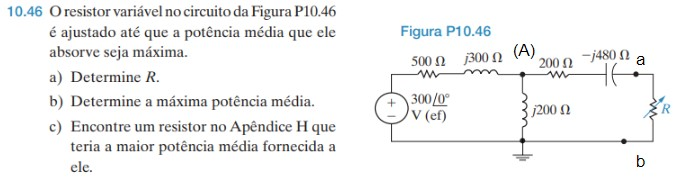
\includegraphics[scale=1.0]{P10.46.jpg}
\end{center}

\subsection*{(a)}

Aplicamos teorema de Thevenin nos terminais $a$ e $b$ mostrados na figura. \\
Começamos calculando a tensão de Thevenin $V_{th}$, abrindo os terminais $a$ e $b$. Nesse caso, temos apenas a malha à esquerda
do nó essencial (A). Assim, aplicando análise de malhas nessa malha, temos

\[ -300 + 500I + j300I + j200I = 0 \]

\[ I(500 + j300 + j200) = 300 \]

\[ I = \frac{300}{500 + j500} = 0,3 + j0,3 \un{A} = 424,25\phase{45^{\circ}} \un{mA}\]

Assim, a tensão $V_A = V_a$ é dada por   

\[ V_a = j200 \cdot I = 200\phase{90^{\circ}} \;\Omega \cdot 424,25\phase{45^{\circ}} \un{mA}\]

\[ V_a = V_{ab} = V_{th} = 84,85\phase{135^{\circ}} \un{V}\]

Agora curto-circuitamos os terminais $a$ e $b$ para achar a corrente $I_{sc}$. Nesse caso, aplicamos análise nodal no nó
essencial (A), obtendo

\[ \frac{V_A - 300}{500 + j300} + \frac{V_A}{j200} + \frac{V_A}{200 - j480} = 0 \]

\[ V_A\left(\frac{1}{500 + j300} + \frac{1}{j200} + \frac{1}{200 - j480}\right) = \frac{300}{500 + j300} \]

\[ V_A = \frac{\frac{300}{500 + j300}}{\frac{1}{500 + j300} + \frac{1}{j200} + \frac{1}{200 - j480}} \]

\[ V_A = \frac{0,4412 - j0,2647}{0,00221 - j0,00410} \]

\[ V_A = 110,46\phase{30,71^{\circ}} \un{V} \]

Assim, temos a corrente de curto-circuito dada por

\[ I_{sc} = \frac{V_A}{200 - j480} = \frac{110,46\phase{30,71^{\circ}}}{200 - j480} = 212,42\phase{98,09^{\circ}}\un{mA} \]

Conhecido $V_{th}$ e $I_{sc}$, temos a impedância de Thevenin dada por

\[ Z_{th} = \frac{V_{th}}{I_{sc}} = 399,5\phase{36,91^{\circ}} \;\Omega \]

Para que tenhamos a máxima transferência de potência, precisamos que

\[ R = (Z_{th})^* \]

Contudo, como a resistência $R$ é puramente real, temos que a condição de máxima potência é

\[ R = |(Z_{th})^*| \]

Portanto, 

\[ \boxed{R = 399,5 \;\Omega} \]

\subsection*{(b)}

Usando o circuito equivalente Thevenin, sabemos que a corrente que passa pelo resistor $R$ é

\[ I_R = \frac{V_{th}}{R + Z_{th}} \]

\[ I_R = \frac{84,85\phase{135^{\circ}}}{399,5 + 319,43 + j239,92} = \frac{84,85\phase{135^{\circ}}}{718,93 + j239,92} \]

\[ I_R = 111,95\phase{116,54^{\circ}} \un{mA} \]

Assim, a potência $P_R$ no resistor de carga é

\[ P_R = R \cdot |I_{R}|^2 \]

\[ \boxed{P_R = 5 \un{W}} \]

\subsection*{(c)}

O resistor com valor comercial mais próximo do valor calculado de $R = 399,5 \;\Omega$ é o resistor de

\[ \boxed{R_c = 390 \;\Omega} \]



